% This must be in the first 5 lines to tell arXiv to use pdfLaTeX, which is strongly recommended.
% In particular, the hyperref package requires pdfLaTeX in order to break URLs across lines.

\documentclass[11pt]{article}
\bibliographystyle{plainnat}
\usepackage{booktabs}
% Change "review" to "final" to generate the final (sometimes called camera-ready) version.
% Change to "preprint" to generate a non-anonymous version with page numbers.
\usepackage[final]{neurips_2024}
\usepackage{hyperref} 
% Standard package includes
\usepackage{times}
\usepackage{latexsym}
\usepackage{adjustbox}
\usepackage{multirow}
% For proper rendering and hyphenation of words containing Latin characters (including in bib files)
\usepackage[T1]{fontenc}
% For Vietnamese characters
% \usepackage[T5]{fontenc}
% See https://www.latex-project.org/help/documentation/encguide.pdf for other character sets

% This assumes your files are encoded as UTF8
\usepackage[utf8]{inputenc}
\usepackage{amsmath}
\usepackage{amsfonts}
\usepackage{float} 
\usepackage{url}
% This is not strictly necessary, and may be commented out,
% but it will improve the layout of the manuscript,
% and will typically save some space.
\usepackage{microtype}

% This is also not strictly necessary, and may be commented out.
% However, it will improve the aesthetics of text in
% the typewriter font.
\usepackage{inconsolata}

%Including images in your LaTeX document requires adding
%additional package(s)
\usepackage{graphicx}
\usepackage{natbib}
\usepackage{mathtools}
\usepackage{algorithm}
\usepackage{algorithmicx}
\usepackage{algcompatible}
\usepackage{algpseudocode}

\usepackage{soul}
\usepackage{nicefrac}
\usepackage{xcolor}   
\hypersetup{
    colorlinks=true,       
    linkcolor=darkgreen,   
    citecolor=darkgreen,   
    urlcolor=blue,         
    pdfborder={0 0 0}  
}
\definecolor{darkgreen}{rgb}{0.0, 0.5, 0.0}

\newcommand{\greenCite}[1]{\textcolor{darkgreen}{\cite{#1}}}
\newcommand{\greenCitep}[1]{\textcolor{darkgreen}{\citep{#1}}}
% If the title and author information does not fit in the area allocated, uncomment the following
%
%\setlength\titlebox{<dim>}
%
% and set <dim> to something 5cm or larger.

\title{Coarse-to-Fine AI Text Detection: Hierarchical Contrastive Learning in Dual Stages}

% Author information can be set in various styles:
% For several authors from the same institution:
% \author{Author 1 \and ... \and Author n \\
	%         Address line \\ ... \\ Address line}
% if the names do not fit well on one line use
%         Author 1 \\ {\bf Author 2} \\ ... \\ {\bf Author n} \\
% For authors from different institutions:
% \author{Author 1 \\ Address line \\  ... \\ Address line
	%         \And  ... \And
	%         Author n \\ Address line \\ ... \\ Address line}
% To start a separate ``row'' of authors use \AND, as in
% \author{Author 1 \\ Address line \\  ... \\ Address line
	%         \AND
	%         Author 2 \\ Address line \\ ... \\ Address line \And
	%         Author 3 \\ Address line \\ ... \\ Address line}

\author{First Author \\
	Affiliation / Address line 1 \\
	Affiliation / Address line 2 \\
	Affiliation / Address line 3 \\
	\texttt{email@domain} \\\And
	Second Author \\
	Affiliation / Address line 1 \\
	Affiliation / Address line 2 \\
	Affiliation / Address line 3 \\
	\texttt{email@domain} \\}

%\author{
	%  \textbf{First Author\textsuperscript{1}},
	%  \textbf{Second Author\textsuperscript{1,2}},
	%  \textbf{Third T. Author\textsuperscript{1}},
	%  \textbf{Fourth Author\textsuperscript{1}},
	%\\
	%  \textbf{Fifth Author\textsuperscript{1,2}},
	%  \textbf{Sixth Author\textsuperscript{1}},
	%  \textbf{Seventh Author\textsuperscript{1}},
	%  \textbf{Eighth Author \textsuperscript{1,2,3,4}},
	%\\
	%  \textbf{Ninth Author\textsuperscript{1}},
	%  \textbf{Tenth Author\textsuperscript{1}},
	%  \textbf{Eleventh E. Author\textsuperscript{1,2,3,4,5}},
	%  \textbf{Twelfth Author\textsuperscript{1}},
	%\\
	%  \textbf{Thirteenth Author\textsuperscript{3}},
	%  \textbf{Fourteenth F. Author\textsuperscript{2,4}},
	%  \textbf{Fifteenth Author\textsuperscript{1}},
	%  \textbf{Sixteenth Author\textsuperscript{1}},
	%\\
	%  \textbf{Seventeenth S. Author\textsuperscript{4,5}},
	%  \textbf{Eighteenth Author\textsuperscript{3,4}},
	%  \textbf{Nineteenth N. Author\textsuperscript{2,5}},
	%  \textbf{Twentieth Author\textsuperscript{1}}
	%\\
	%\\
	%  \textsuperscript{1}Affiliation 1,
	%  \textsuperscript{2}Affiliation 2,
	%  \textsuperscript{3}Affiliation 3,
	%  \textsuperscript{4}Affiliation 4,
	%  \textsuperscript{5}Affiliation 5
	%\\
	%  \small{
		%    \textbf{Correspondence:} \href{mailto:email@domain}{email@domain}
		%  }
	%}

\begin{document}
	\maketitle
	\begin{abstract}
		As the ability of Large Language Models (LLM) to imitate human writing becomes stronger and the diversity of machine texts disguises continuously increases, current AI text detectors have shown vulnerabilities. Among them, a considerable number of detectors are single-stage, relying heavily on the comparison results between final text score and the threshold value for judgment, which has significant vulnerabilities when dealing with strategically disguised machine texts. Given that the current disguise methods can be roughly divided into four levels: character, word, sentence, and paragraph, we targetedly propose a two-stage detector based on hierarchical contrastive learning. The "human" texts filtered out in the first-stage contains real human texts and disguised machine texts, and these samples will be fine-grainedly discriminated through the second-stage detector which applies a hierarchical unsupervised contrastive learning strategy. This multi-stage strategy makes up for the loophole that disguised machine texts can successfully escape the traditional detector after a single detection, and shows excellent robustness in the task of detecting disguised machine texts. In addition, the second-stage detector can be deployed separately on the existing detector as a backup when facing large-scale disguised machine texts attack. Experiments show that our two-stage detector has achieved advanced results, moreover, this detachable and composable approach shows strong flexibility and generalization. We hope that this multi-stage training strategy can inspire new sparks in the field of AI-generated text detection.Our code and dataset will soon be available.
	\end{abstract}
	

	
	\section{Introduction}
	\begin{figure*}
    \centering
    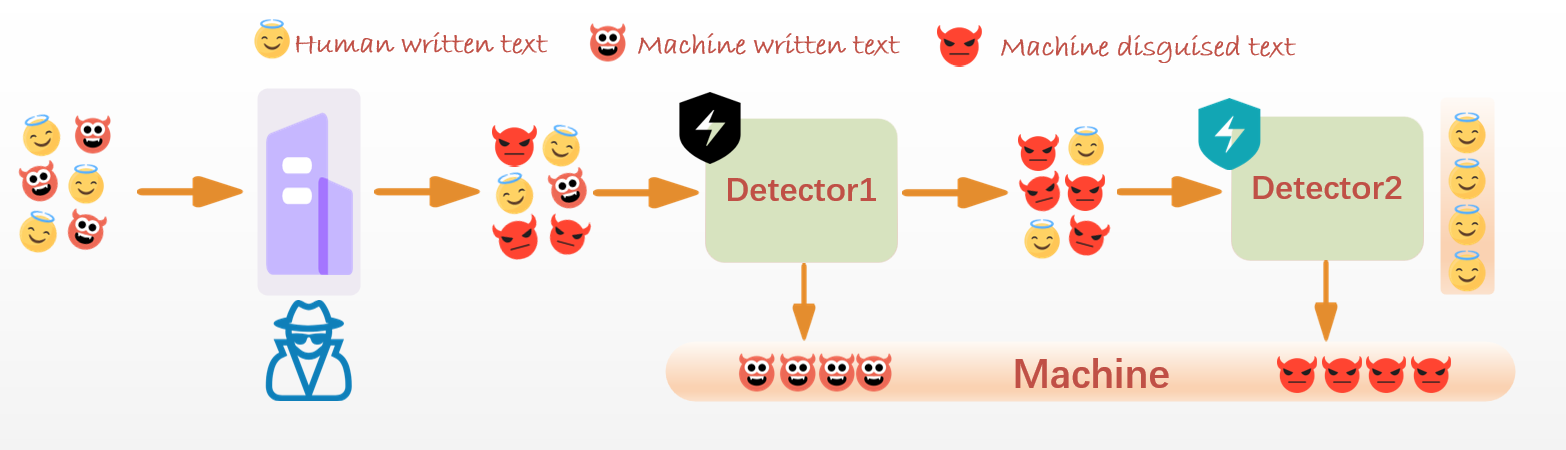
\includegraphics[width=1.0\linewidth]{pics/frame.png}
    \caption{Overview of framework. (a) Machine text disguise. Machine-generated texts may be disguised by attackers to evade detection. We put the original machine texts into the factory for processing and get the disguised machine texts. (b) First-stage detect. The texts are filtered through the first-stage detector, and most of the original machine texts will be filtered out. (c) Second-stage detect. The filtered texts moves to the second-stage detector to get fine-grained recognition.}
\label{fig:method}
\end{figure*}

	The explosive rise of LLMs\greenCitep{Claude2024,deepseekai2025,geminiteam2024geminifamilyhighlycapable} makes it easy for people to get machine-generated texts. However, just as a coin has two sides, new problems emerge when the text generation function of LLMs facilitates people's work and life. Researchers have demonstrated various malicious applications of LLMs, including academic fraud\greenCitep{Perkins2023}, spam generation, and false information dissemination\greenCitep{hazell2023spear,Weidinger2022taxonomy}. In order to prevent machine-generated texts from leaning into the wrong direction, machine-generated text detectors come into being to correct the development of LLMs. Existing detectors include those based on statistics and mathematics\greenCitep{mitchell2023detectgpt,tian2023gptzero}, watermarks\greenCitep{gu2022watermarking,kirchenbauer2023watermark}, classifiers\greenCitep{guo2023simpleai,wang2023seqxgpt}, to name a few. Among them, a considerable number of detectors judge whether the text is generated by the machine based on the comparison of the final text score with a certain threshold. For example, when the test score of a text is greater than 0.5, it is considered to be written by a machine, otherwise it is considered to be written by a human. However, as large quantities of machine texts become easier to obtain and the disguise methods become more and more diverse\greenCitep{zhou2024navigatingshadows,huang2024ai}, it is not enough for detectors to depend solely on the comparison of the final texts score with a certain threshold, and further improvement is needed.

	There are many ways of machine disguise methods at present, such as simulating human spelling errors, word replacement, sentence back translation and so on, which can be roughly divided into four levels: character, word, sentence, and paragraph\greenCitep{zhou2024navigatingshadows}. The vulnerability of detectors in the face of these attacks has also been pointed out by many researchers\greenCitep{dugan2024raid,krishna2024paraphrasing}. Therefore, we believe that it is necessary to conduct a two-stage detection of texts, to detailedly speak, when the scores of texts are within the machine category range, the output is normally machine-generated, and when the texts' scores are within the human category range, the texts may not only be human written, but also disguised machine texts, and a second-stage detection is required. In other words, we add an extra gate to the detector, so that disguised machine texts not only need to pass the first-stage detection, but also have to undergo an extra fine-grained inspection by second-stage detector, which greatly reduces the possibility of machine texts evading detection, thereby improving the robustness of detector in the face of attacks.\\
	Specifically, we propose a two-stage detector. For the first-stage detector, it is trained based on a general classifier framework, while for the second-stage detector, its training data comes from samples judged by the first-stage detector as human writing (including human writing samples and disguised machine samples). In order to further distinguish human samples and machine samples disguised at different levels, we prescribe the right medicine by using hierarchical contrastive learning to learn the similarities and differences between them. Concretely, for machine texts disguised at the same level, their distances in the sample space should be close to each other and far from machine samples disguised at other levels; for machine texts disguised at different levels along with original machine texts, their distances in the sample space should be close to each other and far from human texts; for human-written texts, their distances in the sample space should also be close to each other and far from machine samples. The final result can be obtained by integrating the results of the first-stage detection and the second-stage detection, which shows the vulnerability of the first-stage detector (as a representative of the current common detectors) in the face of diversified attacks, the necessity and effectiveness of the second-stage detection, and the excellent performance of our detector that ultimately exceeds the baseline.
	
	We not only propose a joint detector with good performance, but also provide a new training paradigm for subsequent AI text detectors. The two-stage detector breaks through the previous "one" constraint of AI text detectors, allowing them to be disassembled and deployed separately: if the requirements are not high, the first-stage detector is sufficient; and for existing detectors, the second-stage detector can serve as a backup in the face of large-scale machine disguised texts detection, providing them with a possible patch.
	
	In short, our work is multifaceted and can be summarized as follows:\\
	(1) We use hierarchical contrastive learning to achieve fine-grained distinction between human texts, original machine texts and machine texts disguised at different levels, providing ideas for detector designers to resist the current diverse attacks.\\
	(2) We propose a joint framework for training detectors, and the two-stage detector trained by the framework has achieved excellent robustness in detecting machine texts.\\
	(3) The advantage of the two-stage detector is that it can be deployed separately according to needs, and the second-stage detector can be used as a patch to improve the robustness of existing detectors.
	

	\section{Related Works}
	\subsection{Machine-generated text detectors.}
	In order to prevent machine-generated texts from being abused, numbers of detectors have been proposed by researchers, thus consolidating the defense line of text detection. We classify the existing detectors into the following four categories:\\
	\textbf{Statistical and mathematical based detectors}: Using information entropy, cross perplexity, word frequency statistics and other features to perform zero-shot detection.\greenCite{mitchell2023detectgpt} quantify the difference between machines and humans in word selection via conditional probability curvature.\greenCite{su2023detectllm} apply log-rank information to detect. Open source detecting platform \greenCite{tian2023gptzero,gehrmann2019gltrstatisticaldetectionvisualization} are also included.\\
	\textbf{Watermark based detectors}: Watermark detection algorithms in machine texts detection track the source of generated texts by embedding invisible identifiers. Representative works include:\greenCite{gu2022watermarking,liu2024unforgeablepubliclyverifiablewatermark,hou2024clusteringbasedsemanticwatermark,lu2024entropybasedwatermarking}.Among them,\greenCite{kirchenbauer2023watermark} add a fixed weight to the logit value of the predefined "green word list" and determine whether the text is generated by the model by counting the proportion of green words in the texts.\\
	\textbf{Classifier based detectors}:\greenCite{Chen_2023,miao2024efficientdetection,mireshghallah2024smallerlanguagemodelsbetter,wang2023seqxgpt,liu2024checkgpt} typically employ RoBERTa\greenCitep{liu2019roberta} as the backbone architecture for training supervised binary classifiers. Notable developments are seen in OpenAI's official detection toolkit\greenCitep{solaiman2019releasestrategiessocialimpacts} and RADAR\greenCitep{hu2023radarrobustaitextdetection}, which enhances adversarial robustness against perturbation attacks through paraphrase-based adversarial training.
	\textbf{Other methods based detecors}:\greenCite{soto2024fewshotdetectionmachinegeneratedtext} use style representations,\greenCite{huang2024ai} take advantage of siamese neural network,\greenCite{krishna2024paraphrasing} achieve success through retrieval methods.\greenCite{zhu2023beatllm} innovatively query LLM to detect LLM-generated texts.
	
	
	\subsection{Disguise methods of machine-generated texts}
	Many researchers have pointed out the vulnerability of current detectors, indicating even a small perturbation attack can cause the performance of the detector to drop sharply\greenCitep{zhou2024navigatingshadows,dugan2024raid,krishna2024paraphrasing,liu2024pecola,huang2024ai,wang2024stumblingblocks}. Specifically, \greenCite{liu2024pecola} point out that DetectGPT relies on the threshold setting of the logit regression module (which coincides with our motivation), which is sensitive to the detection results, and the perturbations of deletion, duplication, insertion, and replacement imposed on the test data cause the performance of AI text detector to drop significantly; \greenCite{dugan2024raid} design a variety of perturbations such as local vocabulary replacement, syntactic structure adjustment, semantic preservation rewriting, finding that with only 5\% of the text content being modified, the detection accuracy drops by an average of 37.2\%; \greenCite{zhou2024navigatingshadows} use twelve attacks from four levels of character, word, sentence, and paragraph on a variety of detectors, pointing out that current detectors need to be trained with adversarial texts. Their works show that lacerating the mask of disguised texts is an urgent affair that current detectors need to solve.

	\subsection{Contrastive Learing in Detectors}
	There has been work showing that contrastive learning has excellent performance in the field of natural language processing\greenCitep{cheng2023ml}. MixCSE\greenCitep{Zhang2022mixcse}, SimCSE\greenCitep{gao2021simcse}, VaSCL\greenCitep{zhang2022vascl} use unsupervised contrastive learning framework to enhance the semantic discrimination ability of the model; CoCo\greenCitep{liu2023coco} use supervised contrastive learning to make the model pay more attention to difficult negative samples in low-resource scenarios; \greenCite{soto2024fewshot,guo2024detective} use contrastive learning to distinguish the style features of human and machine writing. By narrowing the distance between positive samples and increasing the distance between negative samples, contrastive learning has shown great potential in training AI content detectors.
	
	
	\section{Model and Methodology}
	In this section, we will introduce our proposed method. Section \ref{sec:framework} will describe machine texts disguise methods and the composition of the detection framework, Section \ref{sec:first_stage} is an illustration of the first-stage detector, and Section \ref{sec:second_stage} is a detailed description of the two-stage detector design and an extended discussion of our motivation for using a two-stage detector along with the "blending the strengths of both" core training ideas.
	
	\subsection{Framework Overview}
	\label{sec:framework}
	\greenCite{zhou2024navigatingshadows,huang2024ai}'s work extensively explore the vulnerability of detectors to different attacks. Based on their work, we classify the existing common attack methods into the following four types,which consistent with \greenCite{zhou2024navigatingshadows}'s summary of present attacks:
	\begin{enumerate}
		\item \textbf{char level}:Attacks at this level include space deletion, space addition\greenCitep{cai2023evadechatgpt}, capitalization typo simulation, punctuation deletion, and random word merging.
		\item \textbf{word level}:Attacks at this level include keyboard spelling errors, which replace characters in similar keyboard positions; swaping adjacent characters, inserting irrelevant characters, and deleting specific characters, thereby simulating human negligence when typing; Word spelling errors, which simulate users' incorrect spelling of words through a predefined spelling error dictionary; Adverb perturbations, which randomly insert relevant adverbs before verbs in the original text; Word replacement, which uses the BERT model\greenCitep{devlin2019bert} to replace words in the text with synonyms.
		\item \textbf{sentence level}:Attacks at this level include adding irrelevant sentences; repeating parts of sentences; randomly selecting sentences for back-translation; and sentence-level replacement, which randomly masks 2 to 5 sentences in the original text and replaces them using the BART-large model\greenCitep{lewis2020bart}.
		\item \textbf{paragraph level}:Attacks at this level include rewriting using the Dipper interpreter\greenCitep{krishna2024paraphrasing}; back-translation using the Helsinki-NLP model\greenCitep{tiedemann2020opus}; and rearrangement of paragraph structure.
	\end{enumerate}
	Given a set of undisguised machine original texts $X=\{x_1,x_2,...,x_k\}$ and human writing texts set $Y=\{y_1,y_2,...,y_k\}$, an attacker with ulterior motives may disguise the original texts of machine at character, word, sentence, or paragraph level to try to evade detection, thus there will be sets of disguised machine texts:\\
  $$
\begin{aligned}
&X_{char} = \{x_{char1}, x_{char2}, \dots, x_{chark}\} \\
&X_{word} = \{x_{word1}, x_{word2}, \dots, x_{wordk}\} \\
&X_{sentence} = \{x_{sent1}, x_{sent2}, \dots, x_{sentk}\} \\
&X_{paragraph} = \{x_{para1}, x_{para2}, \dots, x_{parak}\}
\end{aligned}
$$

	Given a sample space S in real world detection,we have $S = X_{char} + X_{word} + X_{sentence} + X_{paragraph} + X + Y$. For a sample $s \in S$, our goal is to ultimately determine whether it is machine generated. Sample $s$ will first pass through the first-stage detector, the final text's score is compared with the threshold and if it is in the machine range, then the conclusion that $s$ is machine generated is directly output, which indicates that some machine samples are successfully identified by the first-stage detector,which is $s \in X$. If the text is judged to be human written, the text may be real human text or machine written text in disguise, which is $s \in X+Y+X_{char}+X_{word}+X_{sentence}+X_{paragraph}$. Sample $s$ which is judged as human by the first stage will enter the second detector for detection.In the second detector, $s$ will undergo multi-level contrastive learning for fine-grained differentiation, ultimately determining whether $s$ is indeed a disguised machine text.
	
	
	\subsection{First Stage Detector}
	\label{sec:first_stage}
	The first stage detector is a traditional classifier-based detector. Its purpose is to perform coarse-grained screening of input batch text. The first-stage detector can also be used as a representative of the current detector that has not been specially trained with text perturbations. A good first-stage detector should be able to filter out most of the original machine text that has not been disguised. Its loss function is as follows,in which l represents true label,p represents predicted label:
  \begin{equation}
    \begin{aligned}
        \label{eq:loss_ce}
        \mathcal L_{ce}=-\frac{1}{N}\displaystyle\sum_{i=1}^N l_i\cdot log(p_i)+(1-l_i)\cdot log(1-p_i),
    \end{aligned}
\end{equation}
For input $s \in S$, the text encoding $\Phi(s)$, the output is:
\begin{equation}
	\label{ineq:seq_equal}
		Prediction(s) = 
		\begin{cases}
			human, score(\Phi(s))>threshold \\
			machine, scores(\Phi(s)) < threshold
		\end{cases}
	\end{equation}

	
	\subsection{Second Stage Detector}
	\label{sec:second_stage}
	\begin{figure*}
    \centering
    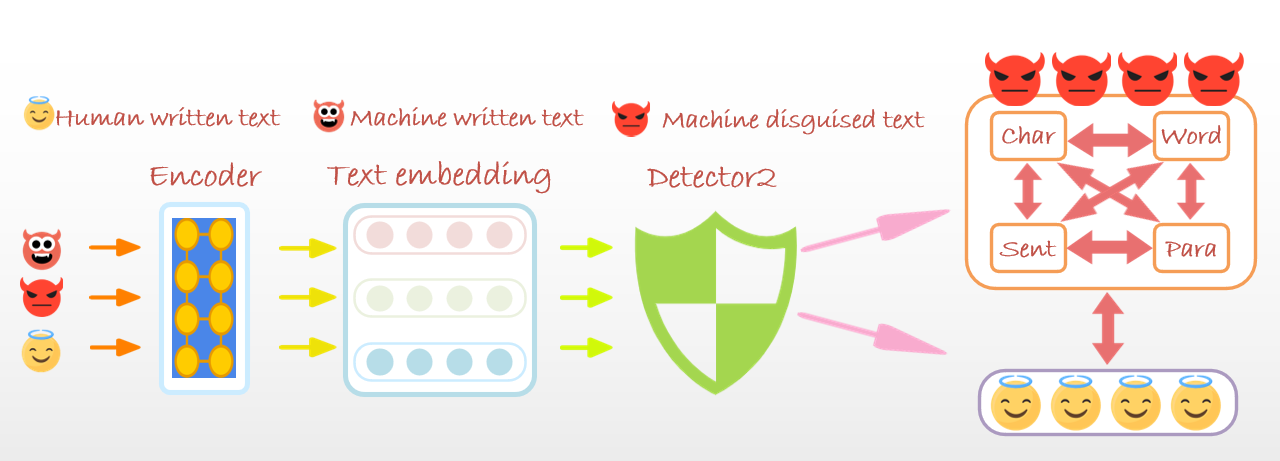
\includegraphics[width=1.0\linewidth]{pics/second-detector.png}
    \caption{Overview of the second stage detector. After the text is encoded by the encoder, it's deeper features are learned through hierarchical contrastive learning strategy, which pulls in the same positive samples and pushes away the negative samples to distinguish human texts and machine texts that have undergone four levels of disguise.}
\label{fig:second-detector}
\end{figure*}
	For the sample set $S^\prime$ entering the second detector, it may be human texts, the original machine texts previously missed by the first-stage detector, or the disguised machine texts that deceived the first-stage detector. Machine texts may use different levels of disguise, accordingly there are three levels of hierarchical contrastive learning in the second-stage detector: machine texts using the same disguise method and machine texts with different disguise methods, machine texts using the same level of disguise method and machine texts with different levels of disguise methods, human texts and machine texts. Given a text label triple $(p, q, l)$, where p represents the disguise method used, q represents the level of the disguise method, and l represents the source of the sample (human or machine), we have the cosine similarity constraints:
	\begin{equation}
    \label{ineq:sim_equal}
    \left\{
    \begin{array}{@{\extracolsep{\fill}}lllll}
      Sim(\Phi(s_1),\Phi(s_2))<Sim(\Phi(s_1),\Phi(s_3)),p(s_1)=p(s_2),p(s_1)\neq p(s_3)\\
      Sim(\Phi(s_4),\Phi(s_5))<Sim(\Phi(s_4),\Phi(s_6)),q(s_4)=q(s_5),q(s_4)\neq q(s_6)\\
      Sim(\Phi(s_7),\Phi(s_8))<Sim(\Phi(s_7),\Phi(s_9)),l(s_7)=l(s_8),l(s_7)\neq l(s_9)\\
    \end{array}
    \right.
    \end{equation}
    where $s_1,s_2,s_3,s_4,s_5,s_6,s_7,s_8,s_9 \in S^\prime$. \\
    For contrastive learning at a specific level, we use the contrastive loss based on the SimCLR framework\greenCitep{chen2020simclr}, which takes the form of a negative logarithmic aggregation function, we have the loss expression eq.\ref{eq:loss_function}, in which $s$ represents targeted sample, $S_{K^+}$ is a set of positive samples, $S_{K^-}$ is a set of negative samples, $\tau$ is the temperature coefficient.
    \begin{equation}
      \begin{aligned}
          \label{eq:loss_function}
           \mathcal L_p= -\log \frac{\exp \left( \sum_{k \in K^+} \frac{s(p, k)}{\tau} / S_{K^+} \right)}{\exp \left( \sum_{k \in K^+} \frac{s(p, k)}{\tau} / S_{K^+} \right) + \sum_{k \in K^-} \exp \left( \frac{s(p, k)}{\tau} \right)}.
      \end{aligned}
      \end{equation}
    We take contrastive loss in label $p$ as example,label $q$ and $l$'s loss are consistent with the above equation.\\
    The final contrastive learning loss should be the sum of the contrastive losses at different levels above, so we have:
    \begin{equation}
      \begin{aligned}
      \label{eq:final_contrastive_loss}
      \mathcal L_{contrastive-tot} = \displaystyle\sum_{i=1}^K l_i \cdot \mathcal L_l + (1 - l_i) \cdot (\mathcal L_p + \mathcal L_q ).
      \end{aligned}
  \end{equation}
  where $l_i$ represents the label $l$ that whether the sample belongs to human or machine, $K$ indicates the sum of all samples entering the second stage detector, and $\mathcal L_l$, $\mathcal L_p$, and $\mathcal L_q$ represents the loss of the second stage detector at above level.\\
  Through hierarchical contrastive loss function propagation, the model can distinguish the differences between machine texts disguised at different levels and the similarities between machine texts disguised at the same level in a fine-grained manner. In order to determine whether the final text is machine-generated, we also introduce the cross entropy loss function eq.\ref{eq:loss_ce} to drive the model to improve performance in the final binary classification task,we have the final loss as:
  \begin{equation}
    \begin{aligned}
        \label{eq:loss_overall}
        \mathcal L_{final-loss}=\mathcal L_{contrastive-tot} + \mathcal L_{ce}.
    \end{aligned}
    \end{equation}
    \textbf{Blending the strengths of both——our two stage training idea:} For the task of detecting human texts and original machine texts, the classification task is simple and direct. The classifier based on cross entropy loss has the advantages of stable optimization process, rapid convergence, and applicability to mutually exclusive scenarios\greenCitep{Dickson2022crossentry,ma2022crossentry,wood2022biasvariance}. Therefore, we choose it as the main body in the first-stage detection, hoping to take advantage of its strengths and quickly filter out the original machine texts without disguise. For the more realistic task of detecting human texts and disguised machine texts, due to the prevalence of LLMs and the various ways of machine text disguise, cross entropy lacks sensitivity to intra-class differences\greenCitep{liu2016largemarginsoftmax,Sun2020circleloss}. Therefore, we introduce hierarchical contrastive learning as the second-stage detector, hoping it can further learn the feature representation of disguised machine texts and human texts.\\
		In general, the first-stage detector quickly and roughly screens texts, solving the problem that the detector based on contrastive learning has high training computational overhead when directly facing large-scale text detection and has limited learned human text feature representation when facing data imbalance\greenCitep{liu2016largemarginsoftmax,sohn2016contrasive}. The detector based on hierarchical contrastive learning, in turn, improves the lack of robustness to fine-grained features of the detector based on cross entropy loss. Therefore, our two-stage detector can achieve better performance in whether detecting human texts and original machine texts or detecting human texts and disguised machine texts. Our experimental results also confirm the correctness of this idea of "blending the strengths of both".
	\section{Experiments}
	In this section, we will introduce the experimental process. Section \ref{sec:dataset} will introduce the dataset we used, Section \ref{sec:metrics} will introduce the evaluation metrics we use to evaluate the model, and Section \ref{sec:baseline} will introduce the existing baseline detectors we compare with.
	\subsection{Datasets}
	\label{sec:dataset}
	We use three datasets that are widely used for detector training and detection. Detailed dataset information in Appendix \ref{subsec:dataset_appendix}. \\
	\textbf{CheckGPT}\greenCitep{liu2024checkgpt}: This dataset contains 900,000 samples, generated by ChatGPT based on prompts, covering multiple fields such as news, reviews, and literatures.\\
	\textbf{HC3}\greenCitep{guo2023simpleai}: A high-quality dataset specifically for fine-tuning dialogue models, containing QA question-answer pairs in multiple fields, each question corresponds to at least one human answer and one machine-generated answer, focusing on multiple open-ended questions such as finance and medicine.\\
	\textbf{SeqXGPT-Bench}\greenCitep{wang2023seqxgpt}: A benchmark dataset designed specifically for sentence-level AI generated text detection tasks, containing text generated from multiple LLMs (such as GPT-2, GPT-Neo, GPT-J, LLaMa, and GPT-3). The dataset uses feature alignment design to align word-level log probabilities to a common vocabulary.

	\subsection{Evaluation metrics}
	\label{sec:metrics}
	In order to systematically and thoroughly evaluate our work and the work of others, we use Accuracy(ACC), F1-score(F1), and Recall (which is further divided into machine-recall and human-recall) as the standard. ACC: The proportion of correctly predicted samples to the total number of samples, which directly reflects the overall prediction accuracy of the model, but may be distorted when the categories are unbalanced; Recall: The proportion of correctly predicted samples among samples that are actually positive, which measures the model's coverage of positive samples, but may have a high false alarm rate; F1: The harmonic average of precision and recall, which balances Precision and Recall and avoids the one-sidedness of a single indicator. We use the three in combination in the hope of evaluating model performance more comprehensively.
	
	\subsection{Baseline Detectors}
	\label{sec:baseline}
	To verify the effectiveness of our method, we select the following five representative detectors as baselines and compare them with our two-stage detector. Considering that machine texts may be disguised in reality, we specially select three baseline detectors that have gone through adversarial training and text perturbation training.\\
	\textbf{SimpleAI}\greenCitep{guo2023simpleai}: Fine-tune the pre-trained RoBERTa model, filter the patterned words in the training data to improve generalization ability, and add sentence-level data to enable the model to capture local features.\\
	\textbf{Watermark}\greenCitep{kirchenbauer2023watermark}: The watermark embeds the signal by biasing the "green token list" at generation time, and the detector counts the actual number of green tokens in the texts. It is completely independent of the generation model, avoiding the overhead of traditional model training while ensuring the robustness and interpretability of the detection.\\
	\textbf{CoCo}\greenCitep{liu2023coco}:By constructing a coherence graph to capture the entity interaction structure of the text and introducing a supervised contrastive learning framework, the model's understanding of language patterns is enhanced.\\
	\textbf{RADAR}\greenCitep{hu2023radarrobustaitextdetection}: Using the adversarial learning framework of generator and discriminater along with some instruction tuning, model shows excellent robustness and transferability.\\
	\textbf{PECOLA}\greenCitep{liu2024pecola}: The noise introduced by random perturbations is reduced through selective perturbation strategies, the key features of the text are retained, and the contrastive learning strategy is further used to enhance the robustness.\\

	\section{Results and Analysis}
	In this section we present our experimental results and analyze them. Specifically, we will first show the refinement of our detector in the task of detecting human texts and original machine text, then we will show the robustness of our detector in the more realistic task of detecting disguised machine text, and finally we will explore the "patch effect" of our two-stage strategy on existing detectors.
	\begin{table*}[ht]
		\centering
		\resizebox{\textwidth}{!}{ 
		\renewcommand{\arraystretch}{1.1}
		\begin{tabular}{llccccc}
		\toprule
		\multirow{2}{*}{Dataset} & \multirow{2}{*}{Detectors} & \multicolumn{5}{c}{Metrics} \\
		\cmidrule(lr){3-7}
		& & Human-recall & Machine-recall & Recall & F1 & ACC \\
		\midrule
		
		\multirow{6}{*}{CheckGPT} 
		& SimpleAI & 90.21 & 87.49 & 88.85 & \underline{88.79} & \underline{88.80} \\
		& Watermark & \underline{96.65} & \underline{97.48} & \textbf{97.06} & 72.26 & 75.69\\
		& CoCo & \textbf{97.42} & 72.38 & 84.90 & 85.97 & 84.55  \\
		& PECOLA & 94.69 & 75.23 & 84.96 & 84.51 & 84.58 \\
		& RADAR & 68.41 & 58.11 & 63.26 & 62.05 & 63.05 \\
		& Two-stage & 87.72 & \textbf{98.94} & \underline{93.33} & \textbf{92.89} & \textbf{93.55}  \\
		\cline{1-7}
		
		\multirow{6}{*}{HC3}
    & SimpleAI & 95.66 & 89.98 & 94.32 & 94.31 & 94.32 \\
    & Watermark & 90.71 & 98.78 & 94.75 & 95.13 & 94.88  \\
    & CoCo & \underline{99.58} & 99.05 & \underline{99.31} & 98.30 & \underline{98.42} \\
    & PECOLA & 97.58 & \underline{99.14} & 98.36 & \underline{98.35} & 98.36 \\
    & RADAR & 84.86 & 94.28 & 89.57 & 90.39 & 89.57 \\
    & Two-stage & \textbf{99.74} & \textbf{99.82} & \textbf{99.78} & \textbf{99.78} & \textbf{99.80} \\
    \cline{1-7}
    
    \multirow{6}{*}{SeqXGPT}
    & SimpleAI & \underline{93.52} & \underline{95.25} & \underline{94.38} & \underline{94.37} & \underline{94.37} \\
    & Watermark & none & none & none & none & none \\
    & CoCo & 91.74 & 72.97 & 82.36 & 79.54 & 80.67 \\
    & PECOLA & 90.35 & 77.72 & 84.04 & 84.04 & 84.13 \\
    & RADAR & 75.99 & 46.31 & 61.15 & 54.16 & 61.37 \\
    & Two-stage & \textbf{94.35} & \textbf{99.04} & \textbf{96.70} & \textbf{96.64} & \textbf{96.66} \\
		\bottomrule
		\end{tabular}
		}
		\caption{Performance results of different models across datasets without disguise.The best number is highlighted in \textbf{bold}, while the second best one is \underline{underlined}, other tables are the same.}
		\label{tab:combined_results}
		\end{table*}

		In order to better illustrate the effectiveness of our method, we retrain the existing baseline detectors on the three datasets of CheckGPT, HC3, and SeqXGPT according to the method described in their papers and compare them with our detector to verify the effectiveness and compatibility of our method. Among them, RADAR does not provide source code, so we use the API they provide. In addition, the watermark-based detector does not need to be trained, and its processing work is to add watermarks to the input dataset. We first conduct extensive tests on undisguised machine texts and human texts. The results are shown in Table \ref{tab:combined_results}. Our detector and the existing baseline detectors achieve good results on the three datasets. For the HC3 and SeqXGPT datasets, our method outperforms all baseline detectors in five evaluating metrics. For the CheckGPT dataset, we achieve the best in machine-recall, F1, and ACC, and also achieve the second best in overall recall. Further, using the comprehensive evaluating metric of F1 to illustrate, our detector is 4.1\% higher than the second place on the CheckGPT dataset and 2.27\% higher than the second place on the SeqXGPT dataset. For the HC3 dataset, although it is released relatively early and the recognition difficulty may be relatively low, all baseline detectors perform well, our method still achieves a certain breakthrough, 1.43\% higher than the second place. The above experimental results show that the cross-data adaptability of our two-stage framework is commendable, and acquires the most advanced performance in the early and simple task of detecting original machine texts and human texts.

		\begin{table*}[ht]
			\centering
			\resizebox{\textwidth}{!}{ 
			\renewcommand{\arraystretch}{1.1}
			\begin{tabular}{llccccc}
			\toprule
			\multirow{2}{*}{Dataset} & \multirow{2}{*}{Detectors} & \multicolumn{5}{c}{Metrics} \\
			\cmidrule(lr){3-7}
			& & Human-recall & Machine-recall & Recall & F1 & ACC \\
			\midrule
			
			\multirow{6}{*}{CheckGPT} 
			& SimpleAI & 88.55 & 90.59 & \underline{89.57} & 70.19 & 90.50 \\
			& Watermark & 53.32 & \underline{99.82} & 76.54 & 69.56 & 56.22 \\
			& CoCo & \textbf{97.58} & 73.68 & 85.63 & \textbf{98.21} & \underline{96.60}  \\
			& PECOLA & \underline{93.45} & 83.55 & 88.5 & 62.64 & 83.98 \\
			& RADAR & 84.27 & 60.89 & 72.71 & 75.35 & 61.94 \\
			& Two-stage & 92.19 & \textbf{99.98} & \textbf{96.08} & \underline{95.71} & \textbf{99.63}  \\
			\cline{1-7}
			
			\multirow{6}{*}{HC3}
			& SimpleAI & 43.34 & \underline{99.82} & 71.58 & 79.25 & \underline{96.44} \\
			& Watermark & 52.74 & 99.32 & 76.03 & 69.05 & 55.16 \\
			& CoCo & \underline{92.36} & 23.99 & 58.18 & \underline{95.09} & 94.44 \\
			& PECOLA & 24.80 & 96.63 & 60.72 & 65.09 & 94.70 \\
			& RADAR & 76.27 & 82.12 & \underline{79.20} & 89.40 & 81.75 \\
			& Two-stage & \textbf{92.53} & \textbf{99.98} & \textbf{96.26} & \textbf{95.99} & \textbf{99.52} \\
			\cline{1-7}
			
			\multirow{6}{*}{SeqXGPT}
			& SimpleAI & 64.13 & \underline{99.34} & 81.74 & 86.18 & 97.04 \\
			& Watermark & none & none & none & none & none \\
			& CoCo & \underline{88.63} & 98.68 & \underline{93.65} & \underline{93.06} & \underline{98.16} \\
			& PECOLA & 24.67 & 98.70 & 61.69 & 65.60 & 93.87 \\
			& RADAR & 76.27 & 57.27 & 66.77 & 72.08 & 58.51 \\
			& Two-stage & \textbf{94.94} & \textbf{99.52} & \textbf{97.23} & \textbf{94.02} & \textbf{99.21} \\
			\bottomrule
			\end{tabular}
			}
			\caption{Performance results of different models across datasets under disguise.}
			\label{tab:combined_results_attacked}
			\end{table*}

			To further illustrate that our two-stage training paradigm can train a more robust detector, we perturb the machine texts in the CheckGPT, HC3, and SeqXGPT datasets at different levels, and retrain the baseline detector based on the perturbed dataset to compare with our detector. The experimental results are shown in Table \ref{tab:combined_results_attacked}. The results show that our detector has achieved State-Of-The-Art(SOTA) performance on the three perturbed datasets. In terms of recall, F1, and ACC, our detector is 17.6\%, 0.93\%, and 3.08\% higher than the second place on the HC3 dataset, and 3.58\%, 0.96\%, and 1.05\% higher than the second place on the SeqXGPT dataset. On the CheckGPT dataset, recall and ACC are both the first place, and F1 also reaches the runner-up performance. Furthermore, for the detector CoCo, which also has outstanding performance, although its performance on the CheckGPT dataset is comparable to ours, it relies on the extraction of entities in the texts and the construction of a coherence graph. If the machine texts are relatively concise and short, its performance will suddenly drop because the model cannot build coherence graphs. For example, in our experiments on the HC3 dataset, we find that 10,083 out of 24,000 data do not have corresponding coherence graphs, which leads to a sudden collapse of CoCo's machine-recall metric (23.99\%). Our detector performes well on all three datasets, and demonstrates excellent generalization and robustness in the more realistic task of detecting disguised machine texts and human texts.

			\begin{table*}[ht]
				\centering
				\resizebox{\textwidth}{!}{ 
				\renewcommand{\arraystretch}{1.1}
				\begin{tabular}{llccccc}
				\toprule
				\multirow{2}{*}{Type} & \multirow{2}{*}{Detectors} & \multicolumn{5}{c}{Metrics} \\
				\cmidrule(lr){3-7}
				& & Human-recall & Machine-recall & Recall & F1 & ACC \\
				\midrule
				
				\multirow{2}{*}{Original} 
				& Single & \textbf{89.48} & 92.25 & 90.86 & 90.45 & 91.44 \\
				& Joint & 88.13 & \textbf{98.99} & \textbf{93.56} & \textbf{93.15} & \textbf{93.77}\\
				\cline{1-7}
				
				\multirow{2}{*}{Attacked}
				& Single & \textbf{86.90} & 94.13 & 90.52 & 55.78 & 93.81 \\
				& Joint & 85.91 & \textbf{99.80} & \textbf{92.86} & \textbf{90.39} & \textbf{99.18}  \\
				
				\bottomrule
				\end{tabular}
				}
				\caption{Performance results of "patching" results.}
				\label{tab:patch_results}
				\end{table*}
				We further explore the effect of our framework in "patching" existing detectors, given that the first-stage detector plays an important role in the overall detection effect, its initial screening of data directly affects the training and detection of the second-stage detector. We replace the first-stage detector based on traditional classification loss with a detector based on supervised contrastive learning, the framework is consistent with \greenCite{Chen2022contastive}'s work,we have:
				\begin{equation}
					\label{ineq:newfirst_function}
					\begin{aligned}
						\mathcal{L}_{con} = -\sum_{s_t \in \mathcal{S}} \frac{1}{c} \log \left( 
							\frac{
									\sum\limits_{\substack{l_r=l_t}} \exp(z_t \cdot z_r / \tau)
							}{
									\sum\limits_{\substack{l_r=l_t}} \exp(s_t \cdot s_r / \tau) + \sum\limits_{l_{r'} \neq l_t} \exp(s_t \cdot s_{r'} / \tau)
							} \right)
					\end{aligned}
					\end{equation}
				where $s$ represents sample, $l$ represents label, $c$ represents the number of samples entering the first stage detector, $\tau$ is the temperature coefficient.
				The final loss function is:
				\begin{equation}
					\label{eq:newfirst_final}
					\begin{aligned}
						\mathcal{L}_{final} = \mathcal{L}_{con} + \mathcal{L}_{ce}
					\end{aligned}
				\end{equation}

				Results are shown in Table \ref{tab:patch_results}. For the existing detectors based on contrastive learning, the F1 reaches 90.45\% and the ACC reaches 91.44\% in the task of detecting human texts and original machine texts, which shows that a relatively ideal effect has been achieved in the first screening and classification of texts. On this basis, we further use our second-stage detector to play the role of the second gate in the hope of achieving a more refined effect. The results are consistent with our expectations. The patched detector further improves the F1 to 93.15\% and the ACC to 93.77\%. Considering that many machine texts in real life often use disguised methods to try to evade the detection of detectors, our patch further improves the recall and ACC for the task of detecting human texts and disguised machine texts. The recall and ACC of machine texts reached nearly perfect 99.80\% and 99.18\%, indicating that the detector can almost completely identify disguised machine texts. For the F1 score, the detector without the patch only has 55.78\%, which shows that it is very sensitive to disguised texts. A large number of machine texts are misjudged as human, resulting in performance degradation. However, using our patch, a second checkpoint is set up in time to capture these disguised texts that bypass detection, and the F1 score is increased by a huge span of 34.61\% to 90.39\%. This further proves our original intention of using two-stage detection: To give the existing detector robustness when facing large-scale machine disguised texts, and further improve its recognition ability of machine texts so that it can effectively capture both original and disguised texts. Overall, by applying our patch, we achieve a significant improvement in most evaluation metrics, with only a minor sacrifice of 1\% in human texts recall, resulting in a substantial overall performance optimization.
	
	\section{Ablation Studies}
	In this section, we will introduce ablation experiments and systematically evaluate the effects of each component. We first split the two-stage detector and apply it separately to the dataset to explore the impact of the composition of each component on the overall effect. Moreover, we train the two detectors directly on the dataset, aiming to verify the effect of "1+1>2".
	\begin{table*}[ht]
		\centering
		\resizebox{\textwidth}{!}{ 
		\renewcommand{\arraystretch}{1.1}
		\begin{tabular}{llccccc}
		\toprule
		\multirow{2}{*}{Type} & \multirow{2}{*}{Detectors} & \multicolumn{5}{c}{Metrics} \\
		\cmidrule(lr){3-7}
		& & Human-recall & Machine-recall & Recall & F1 & ACC \\
		\midrule
		
		\multirow{2}{*}{Original} 
		& First & 88.75 & 92.30 & 90.52 & 90.07 & 90.60 \\
		& Second & \textbf{97.29} & 77.00 & 87.15 & 63.88 & 47.18\\
		& Combined & 87.72 & \textbf{98.94} & \textbf{93.33} & \textbf{92.89} & \textbf{93.55}\\ 
		\cline{1-7}
		
		\multirow{2}{*}{Attacked}
		& First & 86.90 & 94.13 & 90.52 & 55.78 & 93.81 \\
		& Second & \textbf{96.82} & 82.52 & 89.67 & 8.50 & 5.15  \\
		& Combined & 92.19 & \textbf{99.98} & \textbf{96.08} & \textbf{95.71} & \textbf{99.63}\\
		\bottomrule
		\end{tabular}
		}
		\caption{Results of ablation. Original means datasets are unprocessed, while Attacked means datasets are disguised. First represents first-stage detector, Second represents second-stage detector, Combined represents the two-stage detector.}
		\label{tab:ablation_results}
		\end{table*}

		Taking the CheckGPT dataset as an example. First, we directly apply the first-stage detector, the second-stage detector, and the joint detector to the two tasks of detecting human texts and original machine texts (origin), detecting human texts and disguised machine texts (second). The results are shown in Table \ref{tab:ablation_results}. For the first task, the first-stage detector performes well overall, which confirms its applicability and practicality in the simple binary classification task of detecting human texts and original machine texts. The second-stage detector performes relatively averagely, with an F1 of 63.88\% and an ACC of only 47.18\%. This phenomenon is well explained: the second-stage detector is trained with samples screened by the first-stage detector as data set. If it is directly applied to the original texts detection, the effect may not be satisfactory. This is also the reason why the F1 and ACC scores of the second-stage detector plummets in Task 2. For task 2, although the first-stage detector bears a good recall rate, combined with the imbalance of the dataset under this task (the disguise methods of machine texts are varied) and its poor performance in F1 score (55.78\%), indicating that it will misjudge a large number of disguised machine texts as human, which is consistent with our expectation that "the robustness of the first-stage detector is fragile when facing large-scale disguised texts", and is one of the reasons why we introduce the two-stage "patch".\\
		Overall, whether it is detecting original machine text or disguised machine text, deleting any component will lead to a decrease in the overall performance of the detector. For the two-stage detector, it is undoubtedly worthwhile to sacrifice the recall rate of human texts slightly in exchange for a significant improvement in the overall performance.

		\begin{table*}[ht]
			\centering
			\resizebox{\textwidth}{!}{ 
			\renewcommand{\arraystretch}{1.1}
			\begin{tabular}{llccccc}
			\toprule
			\multirow{2}{*}{Type} & \multirow{2}{*}{Detectors} & \multicolumn{5}{c}{Metrics} \\
			\cmidrule(lr){3-7}
			& & Human-recall & Machine-recall & Recall & F1 & ACC \\
			\midrule
			
			\multirow{2}{*}{Original} 
			& First & \textbf{88.75} & 92.30 & 90.52 & 90.07 & 90.60 \\
			& Second & 81.10 & 95.23 & 88.16 & 87.09 & 88.40 \\ 
			& Combined & 87.72 & \textbf{98.94} & \textbf{93.33} & \textbf{92.89} & \textbf{93.55}\\ 
			\cline{1-7}
			
			\multirow{2}{*}{Attacked}
			& First & 68.54 & 98.32 & 83.43 & 74.95 & 96.94  \\
			& Second & 77.00 & 99.85 & 88.42 & 85.51 & 97.83   \\
			& Combined & \textbf{92.19} & \textbf{99.98} & \textbf{96.08} & \textbf{95.71} & \textbf{99.63}\\
			\bottomrule
			\end{tabular}
			}
			\caption{Results of ablation, examining the effect of different parts in detail.}
			\label{tab:directly_trained_results}
			\end{table*}

			\begin{figure*}
				\centering
				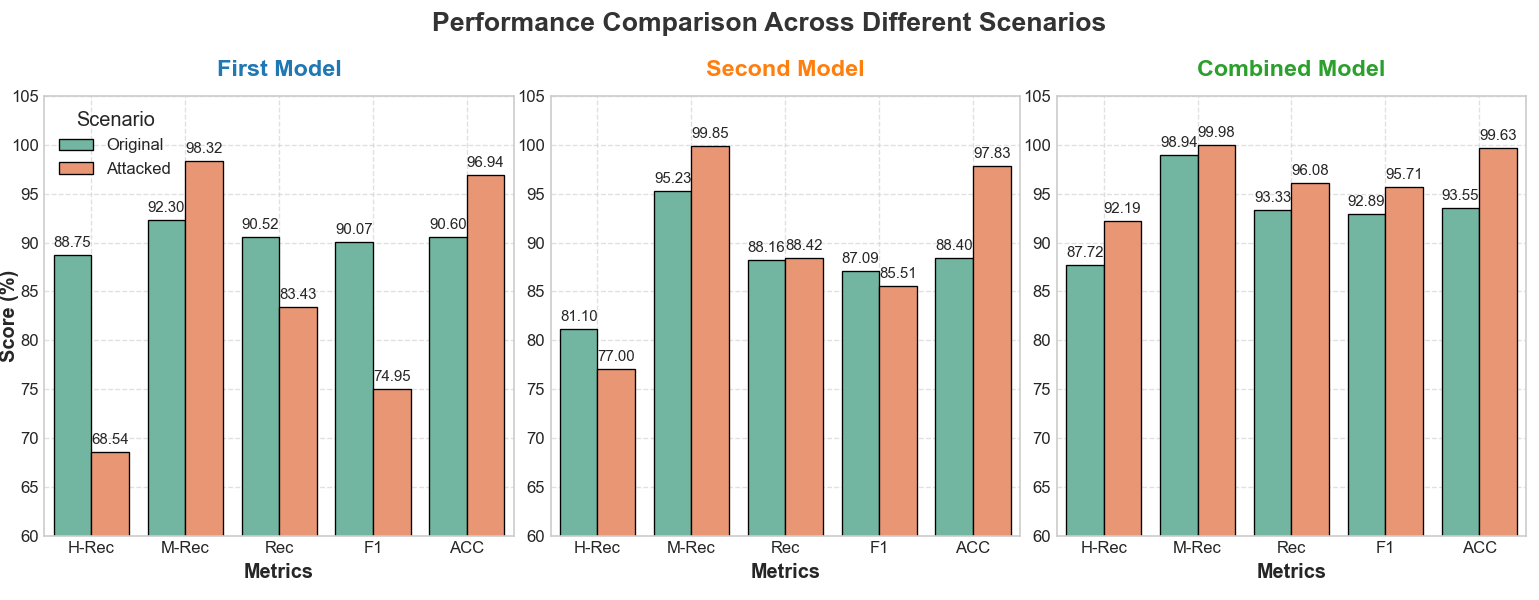
\includegraphics[width=1.0\linewidth]{pics/Figure_1.png}
				\caption{Results of ablation, examining the effect of different parts in detail.}
		\label{fig:ablation_fig2}
		\end{figure*}

		
			To further verify the effectiveness of the two-stage joint training method, we directly trains the first-stage and two-stage detectors on the CheckGPT's human texts and original machine texts, and human texts and disguised machine texts, respectively. The results are shown in Table \ref{tab:directly_trained_results}. For the first-stage detector, even after training with disguised texts, it still has the phenomenon of "wrongly accusing good guys" when detecting disguised machine texts, which reveals the limitations of a single detector in adversarial scenarios --- it can only ensure the stability of some evaluating metrics, but cannot be globally reliable, so it is necessary to fuse multi-dimensional features through a joint detector. For the two-stage detector, in the task of detecting original machine texts, its hierarchical contrastive learning will degenerate into single-level contrastive learning, while in the task of detecting disguised machine texts, its ability to discriminate human texts is slightly weak due to the fact that in the face of a variety of large-scale machine disguised texts in reality, contrastive learning learns limited features of human texts.\\
			Overall,the two-stage detector is the best of the above two detectors,and has a significant increase in evaluating metrics such as F1 and Recall, which shows that our training idea of "blending the strengths of both" is correct and appliable.
			
	\section{Conclusion}
	In this paper, we propose a coarse-to-fine AI generated text detector model and a novel two-stage detector training paradigm. The first-stage detector quickly screens the original machine texts, and the second-stage detector uses hierarchical contrastive learning to carefully distinguish different levels of disguised machine texts. Our detector has achieved SOTA performance in both the task of detecting human texts from original machine texts and the more realistic task of detecting human texts from disguised machine texts, proving the effectiveness of each component and the correctness of the "blending the strengths of both" idea in ablation studies. We hope that this robust detector can better assist AI text detection in real life, and that this two-stage training framework can bring new maps and ideas to researchers in this field.
	
	
	\section{Acknowledgements}
	We sincerely thank all the researchers who have worked in this field and laid the foundation for our work, and we are grateful to all the reviewers, area chairs, and all the scholars who read the paper and provided suggestions.

	\newpage
	\bibliography{custom}
	
	\newpage
	\appendix
	\section{Broader Impacts}
	\label{sec:Impacts}
	The rapid development of LLMs has enabled a large amount of machine-generated texts to be obtained quickly and at low cost. Given that it may lead to academic fraud, phishing emails, the spread of false information and other problems, detecting and monitoring AI-generated texts is undoubtedly a top priority. However, due to the fragility of current AI content detectors and the diversity of text disguise methods, machine texts can easily bypass detection through disguise. Therefore, the development of robust AI content detectors is urgent. Our paper introduces a new robust AI content detector training paradigm, which demonstrates SOTA performance in multiple benchmarks. These advances will bring the green development and use of LLMs with new power. In addition, our second-stage detector can be used as a "patch" to further improve the performance of current detectors when facing large-scale disguised machine texts, which shows that our method has broad prospects for practical application and rich significance.
	
	\section{Limitations and Future Work}
	In this paper, we take into consideration that machine texts may use different disguise methods to evade the detector and thus use hierarchical contrastive learning to strengthen the detector in a targeted manner. However, the original machine texts generated by different models often has certain differences, which may affect the performance of the detector. In addition, we did not introduce some latest disguise strategies (such as adding emoticons to machine texts) and did not train on a larger corpus. In the future, we will continue to work in this direction and further improve the performance of the model.

	\section{Detailed Construction of Dataset}
	\label{subsec:dataset_appendix}
	\begin{table*}[ht]
    \centering
    \begin{minipage}[t]{0.58\textwidth} 
        \centering
        \resizebox{\textwidth}{!}{ 
            \renewcommand{\arraystretch}{1.1}
            \begin{tabular}{lccc}
                \toprule
                \multirow{2}{*}{\large Dataset} & \multirow{2}{*}{\large Train} & \multirow{2}{*}{\large Test} & \multirow{2}{*}{\large Valid} \\
                 & & & \\
                \midrule
                CheckGPT & (2000,2000) & (1921,2078) & (2500,2500) \\
                HC3      & (5000,5000) & (5000,5000) & (2000,2000) \\
                SeqXGPT  & (2467,2533) & (1928,1872) & (1005,995)  \\
                \bottomrule
            \end{tabular}
        }
        \caption{Detailed composition of the dataset for detecting human texts and original machine texts.}
        \label{tab:detailed_original_datasets}
    \end{minipage}
    \hfill 
    \begin{minipage}[t]{0.38\textwidth}
        \centering
        \resizebox{\textwidth}{!}{
            \renewcommand{\arraystretch}{1.1}
            \begin{tabular}{lcc}
                \toprule
                \multirow{2}{*}{Watermark} & \multirow{2}{*}{Human} & \multirow{2}{*}{Machine} \\
                 & & \\
                \midrule
                CheckGPT & 566 & 570 \\
                HC3      & 438 & 538 \\
                SeqXGPT  & 600 & 520 \\
                \bottomrule
            \end{tabular}
        }
        \caption{Detailed composition of the dataset for watermarks.}
        \label{tab:watermark_original_datasets}
    \end{minipage}
\end{table*}

\begin{table*}[ht]
	\centering
	\begin{minipage}[t]{0.58\textwidth} 
			\centering
			\resizebox{\textwidth}{!}{ 
					\renewcommand{\arraystretch}{1.1}
					\begin{tabular}{lccc}
							\toprule
							\multirow{2}{*}{\large Dataset} & \multirow{2}{*}{\large Train} & \multirow{2}{*}{\large Test} & \multirow{2}{*}{\large Valid} \\
							 & & & \\
							\midrule
							CheckGPT & (500,8500) & (1101,23887) & (500,8490) \\
							HC3      & (500,7500) & (1500,22500) & (500,7500) \\
							SeqXGPT  & (500,7500) & (1500,21004) & (500,6494)  \\
							\bottomrule
					\end{tabular}
			}
			\caption{Detailed composition of the dataset for detecting human texts and attacked machine texts.}
			\label{tab:detailed_attack_datasets}
	\end{minipage}
	\hfill 
	\begin{minipage}[t]{0.38\textwidth}
			\centering
			\resizebox{\textwidth}{!}{
					\renewcommand{\arraystretch}{1.1}
					\begin{tabular}{lcc}
							\toprule
							\multirow{2}{*}{Watermark} & \multirow{2}{*}{Human} & \multirow{2}{*}{Machine} \\
							 & & \\
							\midrule
							CheckGPT & 566 & 8550 \\
							HC3      & 438 & 8098 \\
							SeqXGPT  & 600 & 520 \\
							\bottomrule
					\end{tabular}
			}
			\caption{Detailed composition of the attacked dataset for watermarks.}
			\label{tab:watermark_attack_datasets}
	\end{minipage}
\end{table*}
For the simple binary classification task of detecting human texts and original machine texts, the distribution of our samples is shown in Table \ref{tab:detailed_original_datasets}. We ensure the distribution of human texts and machine texts is approximately 1:1. The two-tuple (human, machine) in the table represents the number of human texts and the number of machine texts. For the watermark detector, since it focuses on the hidden singal embedded in the data and does not require training, it only needs to build a test set. While it takes a long time to process the watermark on the dataset, we did not generate a large test set. The data are shown in Table \ref{tab:watermark_original_datasets}.
For the more realistic task of detecting human texts and disguised machine texts, the distribution of our samples is shown in Table \ref{tab:detailed_attack_datasets}. We select 500 human texts and 500 original machine texts from the dataset respectively, and perform 16 disguises methods on the machine texts at the character, word, sentence, and paragraph levels, thereby constructing a perturbation dataset containing human texts, original machine texts, and disguised machine texts. Therefore, the perturbed datasets are mostly composed of machine texts, which are consistent with the current trend of a variety of machine text disguise methods and a flood of generation sources. For the watermark detector, similarly, after the machine texts are injected with the watermark, we disguise them in sixteen different ways and explore whether these disguise strategies will cause the watermark to be covered and invalid. The data distribution is shown in Table \ref{tab:watermark_attack_datasets}.

\section{Comparison of Cross Entropy Loss and Contrastive Learning Loss}
\label{subsec:loss_appendix}
\begin{figure*}
	\centering
	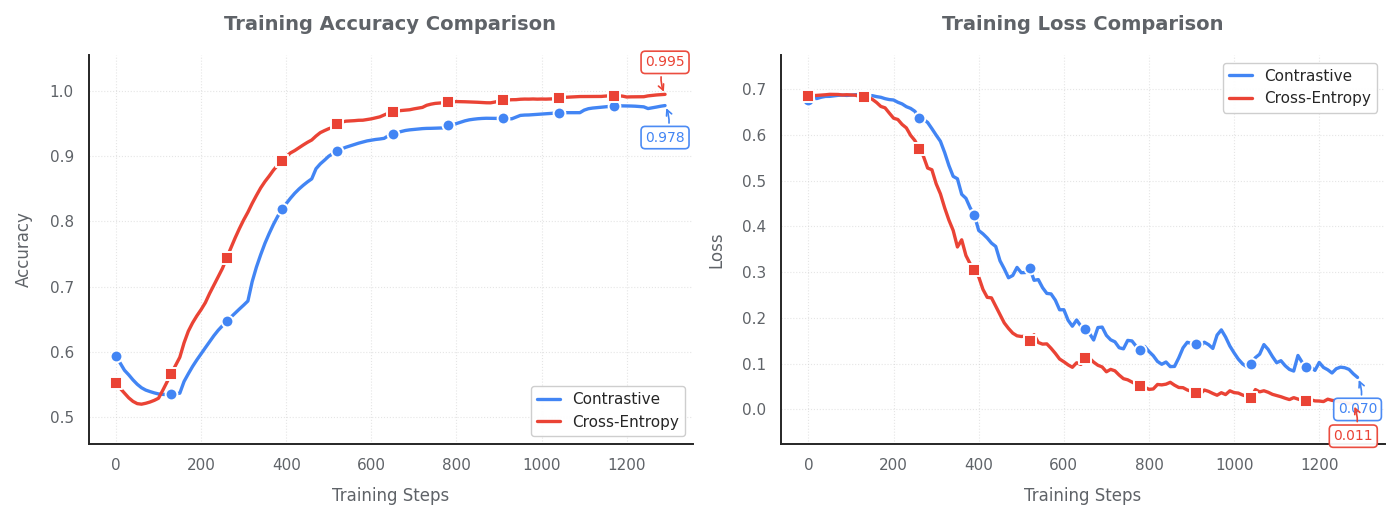
\includegraphics[width=1.0\linewidth]{pics/loss_vs.png}
	\caption{Comparison of contrastive learning and cross entropy on training accuracy and loss.}
\label{fig:loss_compare}
\end{figure*}
We take the SeqXGPT dataset as an example, recording the training accuracy and loss of the two models when using cross entropy loss and contrastive learning loss to train the model respectively, experimental results are shown in Figure \ref{fig:loss_compare}. The results show that the model loss based on cross entropy loss converges faster and is more stable, and for the task of detecting human texts and original machine texts, its training accuracy is higher than that of the model based on contrastive learning, which is one of the reasons why we choose the cross entropy-based classifier model as the first-stage detector.
\end{document}
